% Figure from MATH 591 notes, section 52 (added, not from lecture). Compile with the notes preamble.
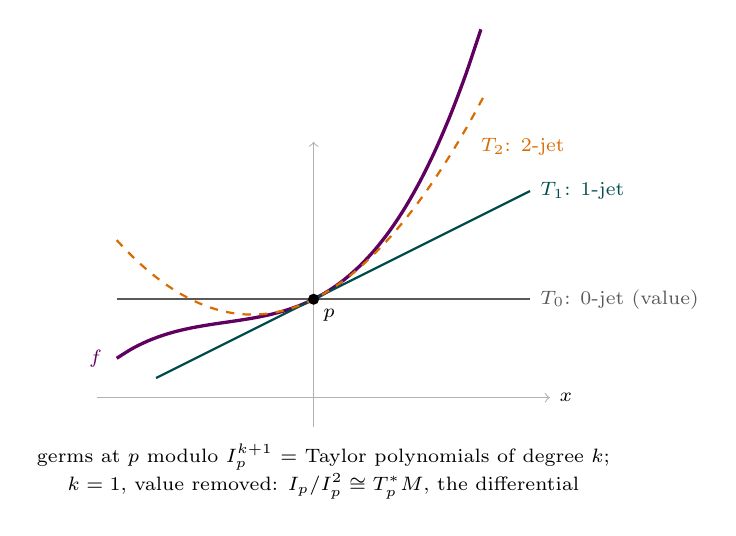
\begin{tikzpicture}[scale=1.25, font=\scriptsize]
\draw[->, gray!60] (-2.2,0) -- (2.4,0) node[right, text=black] {$x$};
\draw[->, gray!60] (0,-0.3) -- (0,2.6);
% f(x) = 1 + 0.5 x + 0.4 x^2 + 0.25 x^3 around p = 0
\draw[violet!75!black, very thick] plot[smooth, domain=-2:1.7] (\x,{1+0.5*\x+0.4*\x*\x+0.15*\x*\x*\x});
\draw[gray!70!black, thick] (-2,1) -- (2.2,1) node[right] {$T_0$: $0$-jet (value)};
\draw[teal!60!black, thick] (-1.6,0.2) -- (2.2,2.1) node[right] {$T_1$: $1$-jet};
\draw[orange!85!black, thick, dashed] plot[smooth, domain=-2:1.75] (\x,{1+0.5*\x+0.4*\x*\x});
\node[orange!85!black, anchor=west] at (1.6,2.55) {$T_2$: $2$-jet};
\node[violet!75!black, anchor=east] at (-2.05,0.4) {$f$};
\fill (0,1) circle (1.6pt); \node[below right] at (0,1) {$p$};
\node[align=center] at (0.1,-0.75) {germs at $p$ modulo $I_p^{k+1}$ $=$ Taylor polynomials of degree $k$;\\ $k = 1$, value removed: $I_p/I_p^2 \cong T_p^*M$, the differential};
\end{tikzpicture}
